\documentclass[spanish, fleqn]{article}
\usepackage{babel}
\usepackage[utf8]{inputenc}
\usepackage{amsmath,amsfonts}
\usepackage{enumitem}
\usepackage[colorlinks, urlcolor=blue]{hyperref}
\usepackage{fourier}
\usepackage[top = 2.5cm, bottom = 2cm, left = 2.5cm, right = 2.5cm]{geometry}
\pagestyle{empty}
\usepackage{tikz}
\usetikzlibrary{positioning,arrows}
\usepackage{pgf}
\usepackage{color}
\tikzset{
every picture/.append style={
  execute at begin picture={\deactivatequoting},
  execute at end picture={\activatequoting}
  }
}


\title{Estructuras Discretas \\
       Actividad Extra \#2 \\
       ``Grafos''}
\author{Andrés  Navarro \\ (201673001-K)}
\date{}

\begin{document}
\maketitle
\thispagestyle{empty}

\section*{Preguntas}
    
\begin{enumerate}
\item Busque y mencione dos ejemplos prácticos donde se utilicen grafos en problemas de la computación.

Dado que los grafos en la computación se usan para representar de forma cómoda relaciones entre objetos, podemos dar como ejemplo el uso de estos para la representación de una red de transporte, pudiendo ser esta un sistema de metros, en donde las relaciones vendrían a ser las conexiones entre las estaciones. Otra aplicación de estos podría ser su uso en problemas de optimización, para establecer conexiones más directas entre objetos.

\item Escriba la definición formal de un grafo y mencione 2 ejemplos indicando que representan los arcos y vértices.

Un grafo consta de un conjunto no vacío de vértices finitos (V) y un conjunto de arcos (E), que corresponden a pares de vértices pertenecientes a V. 

Grafo de relaciones amorosas, en donde los vértices representan a las personas y los arcos, a si estos se han relacionado amorosamente.

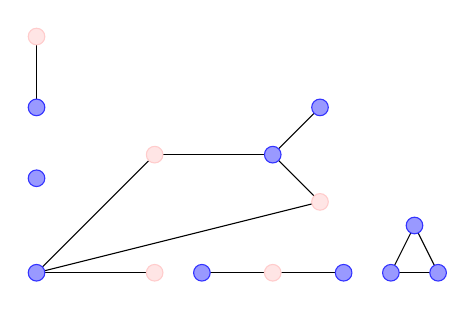
\begin{tikzpicture}[y=.3cm, x=.3cm,font=\normalsize]
\draw (0,0) -- (5,5);
\draw (5,5) -- (10,5);
\draw (0,0) -- (5,0);
\draw (10,5) -- (12,7);
\draw (10,5) -- (12, 3);
\draw (0,0) -- (12, 3);
\draw (0,7) -- (0,10);
\draw (0,4);
\draw (7,0) -- (10,0);
\draw (13,0) -- (10,0);
\draw (15,0) -- (17,0);
\draw (15,0) --(16,2);
\draw (16,2)--(17,0);


;\filldraw[fill=blue!40,draw=blue!80] (0,0) circle (3pt)  ;
\filldraw[fill=pink!40,draw=pink!80] (5,5) circle (3pt)     ;
\filldraw[fill=pink!40,draw=pink!80] (5,0) circle (3pt)     ;
\filldraw[fill=blue!40,draw=blue!80] (10,5) circle (3pt)     ;
\filldraw[fill=blue!40,draw=blue!80] (12,7) circle (3pt)     ;
\filldraw[fill=pink!40,draw=pink!80] (12,3) circle (3pt)     ;
\filldraw[fill=pink!40,draw=pink!80] (0,10) circle (3pt)     ;
\filldraw[fill=blue!40,draw=blue!80] (0,7) circle (3pt)     ;
\filldraw[fill=blue!40,draw=blue!80] (0,4) circle (3pt)     ;
\filldraw[fill=pink!40,draw=pink!80] (10,0) circle (3pt)     ;
\filldraw[fill=blue!40,draw=blue!80] (7,0) circle (3pt)     ;
\filldraw[fill=blue!40,draw=blue!80] (13,0) circle (3pt)     ;
\filldraw[fill=blue!40,draw=blue!80] (15,0) circle (3pt)     ;
\filldraw[fill=blue!40,draw=blue!80] (17,0) circle (3pt)     ;
\filldraw[fill=blue!40,draw=blue!80] (16,2) circle (3pt)     ;

\end{tikzpicture}

Grafo de países colindantes, en donde los vértices representan a los países y los arcos si estos están uno al lado del otro.

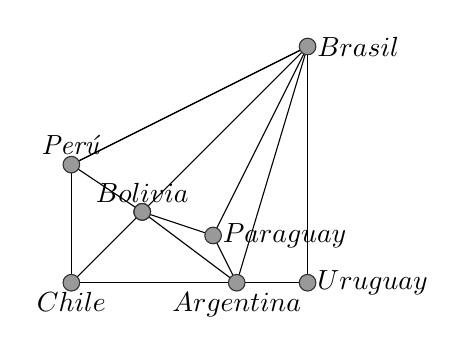
\begin{tikzpicture}[y=.3cm, x=.3cm,font=\normalsize]
\draw (0,0) -- (7,0);
\draw (0,0) -- (0,5);
\draw (0,0) -- (3,3);
\draw (3,3) -- (10,10);
\draw(7,0)--(10,10);
\draw(0,5)--(10,10);
\draw (10,0)--(10,10);
\draw (0,5)--(10,10);
\draw (7,0)--(10,0);
\draw (0,5)--(3,3);
\draw (7,0)--(3,3);
\draw (6,2)--(3,3);
\draw (6,2)--(7,0);
\draw (6,2)--(10,10);

\filldraw[fill=black!40,draw=black!80] (0,0) circle (3pt)   ;
\filldraw[fill=black!40,draw=black!80] (0,5) circle (3pt)    ;
\filldraw[fill=black!40,draw=black!80] (7,0) circle (3pt)    ;
\filldraw[fill=black!40,draw=black!80] (3,3) circle (3pt)  ;
\filldraw[fill=black!40,draw=black!80] (10,10) circle (3pt)  ;
\filldraw[fill=black!40,draw=black!80] (10,0) circle (3pt)  ;
\filldraw[fill=black!40,draw=black!80] (3,3) circle (3pt)  ;
\filldraw[fill=black!40,draw=black!80] (3,3) circle (3pt)  ;
\filldraw[fill=black!40,draw=black!80] (6,2) circle (3pt)  ;

\node [above] at (0,5) {\textit{Perú}};
\node [below] at (0,0) {$Chile$};
\node [right] at (6,2) {$Paraguay$};
\node [right] at (10,0) {$Uruguay$};
\node [above] at (3,3) {$Bolivia$};
\node [below] at (7,0) {$Argentina$};
\node [right] at (10,10) {$Brasil$};
\end{tikzpicture}

\item Invente un grafo con 10 vértices y represéntelo utilizando \emph{lista de adyacencia}, \emph{matriz de adyacencia} y \emph{gráficamente} y luego dibuje un grafo \emph{isomorfo} al grafo que inventó.

\hfill

\hfill

\begin{itemize}
\item Representación gráfica:

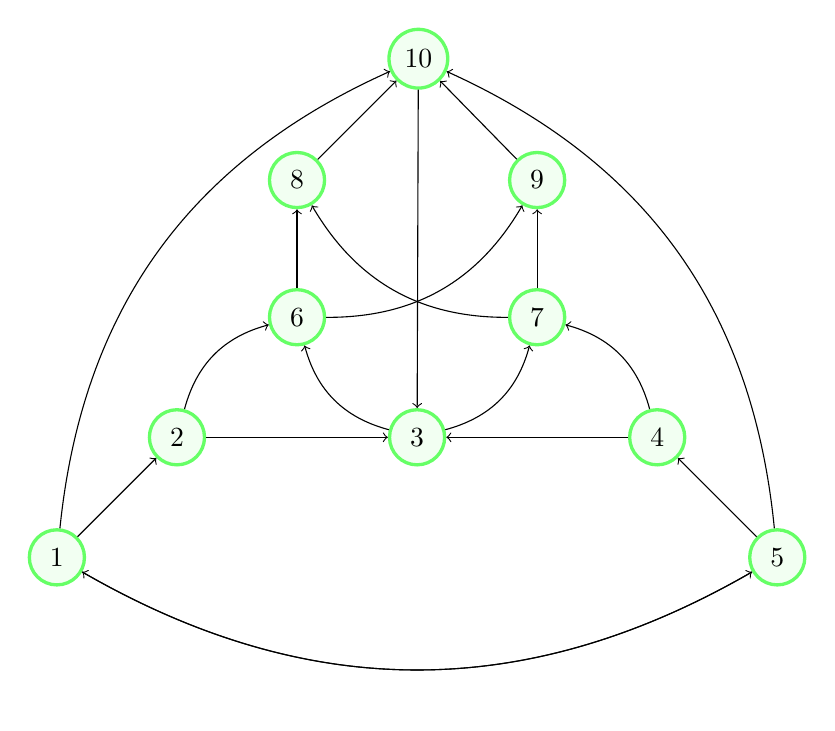
\begin{tikzpicture}[
roundnode/.style={circle, draw=green!60, fill=green!5, very thick, minimum size=7mm}
]

\node[roundnode] (1)       {1};
\node[roundnode] (2)       [above right=of 1] {2};
\node[roundnode] (6)       [above right=of 2] {6};
\node[roundnode] (3)       [below right=of 6] {3};
\node[roundnode] (7)       [above right=of 3]{7};
\node[roundnode] (4) 	  [below right=of 7]{4};
\node[roundnode] (5) 	  [below right=of 4]{5};
\node[roundnode] (8) 	  [above=of 6]{8};
\node[roundnode] (9) 	  [above=of 7]{9};
\node[roundnode] (10) 	  [above right=of 8]{10};
 
\draw [->] (1) -- (2);
\draw [->](1) edge [bend right] (5);
\draw[->] (2) -- (3);
\draw[->] (4) -- (3);
\draw [->] (5) edge [bend right] (10);
\draw [->] (1) edge [bend left] (10);
\draw [->] (9) edge (10);
\draw [->] (8) edge (10);
\draw [->] (5)--(4);
\draw [->] (7) -- (9);
\draw [->] (6)--(8);
\draw [->] (3) edge [bend right] (7);
\draw [->] (3) edge [bend left] (6);
\draw [->] (4) edge [bend right] (7);
\draw [->] (2) edge [bend left] (6);
\draw [->] (5) edge [bend left] (1);
\draw [->] (6) edge [bend right] (9);
\draw [->] (7) edge [bend left] (8);
\draw [->] (10) -- (3);
\end{tikzpicture}

\item Lista de adyacencia:

\begin{tabular}{|c|c|}
\hline
\textbf{V} & \textbf{Ady} \\ \hline
1 & 2,5,10\\ \hline
2 & 3,6\\ \hline
3 & 6,7\\ \hline
4 & 3,7\\ \hline
5 & 1,4,10\\ \hline
6 & 8,9\\ \hline
7 & 8,9\\ \hline
8 & 10\\ \hline
9 & 10\\ \hline
10 & 3\\ \hline
\end{tabular}
\item Matriz de adyacencia:

\begin{tabular}{|c|c|c|c|c|c|c|c|c|c|c|}
\hline
&1&2&3&4&5&6&7&8&9&10\\ \hline
1&0&1&0&0&1&0&0&0&0&1\\ \hline
2&0&0&1&0&0&1&0&0&0&0\\ \hline
3&0&0&0&0&0&1&1&0&0&0\\ \hline
4&0&0&1&0&0&0&1&0&0&0\\ \hline
5&1&0&0&1&0&0&0&0&0&1\\ \hline
6&0&0&0&0&0&0&0&1&1&0\\ \hline
7&0&0&0&0&0&0&0&1&1&0\\ \hline
8&0&0&0&0&0&0&0&0&0&1\\ \hline
9&0&0&0&0&0&0&0&0&0&1\\ \hline
10&0&0&1&0&0&0&0&0&0&0\\ \hline
\end{tabular}

\hfill

\hfill

\hfill

\hfill

\hfill

\hfill

\hfill

\item Grafo isomorfo:

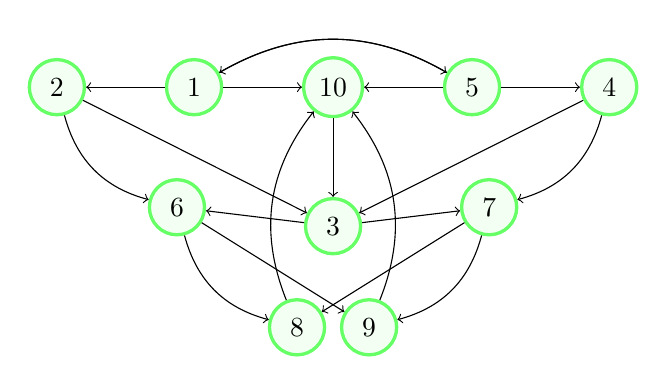
\begin{tikzpicture}[
roundnode/.style={circle, draw=green!60, fill=green!5, very thick, minimum size=7mm}
]

\node[roundnode] (2)       {2};
\node[roundnode] (1)       [right=of 2] {1};
\node[roundnode] (10)       [right=of 1] {10};
\node[roundnode] (5)       [right=of 10] {5};
\node[roundnode] (4)       [right=of 5]{4};
\node[roundnode] (6) 	  [below right=of 2]{6};
\node[roundnode] (8) 	  [below right=of 6]{8};
\node[roundnode] (7) 	  [below left=of 4]{7};
\node[roundnode] (9) 	  [below left=of 7]{9};
\node[roundnode] (3) 	  [below=of 10]{3};
 
\draw [->] (1) -- (2);
\draw [->](1) edge [bend left] (5);
\draw[->] (2) -- (3);
\draw[->] (4) -- (3);
\draw [->] (5) -- (10);
\draw [->] (1) -- (10);
\draw [->] (9) edge [bend right](10);
\draw [->] (8) edge [bend left](10);
\draw [->] (5)--(4);
\draw [->] (7) edge [bend left] (9);
\draw [->] (6)edge [bend right](8);
\draw [->] (3) -- (7);
\draw [->] (3) -- (6);
\draw [->] (4) edge [bend left] (7);
\draw [->] (2) edge [bend right] (6);
\draw [->] (5) edge [bend right] (1);
\draw [->] (6) -- (9);
\draw [->] (7) -- (8);
\draw [->] (10) -- (3);
\end{tikzpicture}
\end{itemize}

\item En la sección \textbf{24.4} aparecen algunas familias especiales de grafos, describa \textbf{informalmente}, es decir, con sus propias palabras, de que se trata cada una de ellas.

\begin{itemize}
\item $P_{n}$: Este grafo posee la característica de que cada uno de sus vértices está, como máximo, conectado con otros dos. Esto significa que, si poseemos una lista de vértices, cada uno podría estar conectado al nodo siguiente, teniendo el primer y último vértice una sola conexión y el resto de ellos con dos conexiones. Posee una forma similar a una hilera.
\item $C_{n}$: Este grafo posee la característica de que su representación gráfica se puede visualizar una figura geométrica. Aquí, si poseemos una lista de vértices, cada uno podría estar conectado al nodo siguiente, pero ahora el último y el primero también estarían conectado entre sí. 
\item $K_{n}$: Este grafo posee la característica de que cada vértice está conectado con todos los demás.
\item $W_{n}$: Este grafo es una modificación del grafo $C_{n}$ en donde este posee un vértice central conectado a todos los demás vértices. 
\item $Q_{n}$: Este grafo posee una cantidad de vértices igual a $2^n$ ya que corresponde a un cubo de grado n. Estos cubos poseen la característica de que se unen entre sí a través de lo que serían sus esquinas, uniendo cada esquina a la que ocupa su misma posición en el otro (u otros cubos), en el caso de que n sea mayor a 3. $Q_0$ corresponde a un punto, $Q_1$ corresponde a una línea y $Q_2$ corresponde a un cuadrado, luego de esto se forman cubos como tal.
\end{itemize}  
\end{enumerate}
\end{document}
